\documentclass[11pt, oneside]{article}
\usepackage{geometry} 
\geometry{letterpaper} 
\usepackage{graphicx}
\usepackage{minted}
\usepackage{mathtools}
\usepackage[T1]{fontenc} 
\usepackage{lmodern}
\usepackage{listings} 
\usepackage{float}
\usepackage{makeidx}
\usepackage{minted}
\usepackage[hypcap]{caption}
\usepackage{pdflscape}
\newcommand{\cvl}{\ttbf{C VSIPL}}
\newcommand{\cvpp}{\ttbf{C++ VSIPL}}
\newcommand{\pyjv}{{\ttbf{pyJvsip}}}
\newcommand{\ttbf}[1]{{\ttfamily \bfseries #1}}
\newcommand{\jv}{{\ttbf{JVSIP}}}
\newcommand{\Blk}{\ttbf{Block}}
\newcommand{\blk}{\ttbf{block}}
\newcommand{\Vw}{\ttbf{View}}
\newcommand{\vw}{\ttbf{view}}
\title{JVSIP Data Model}
\author{Randall Judd}
\begin{document}
\maketitle
\section*{Introduction}
In this document I am proposing a standard data model for VSIPL. To be fair this is my notion of what a data model is. If there is some formal document describing what a data model is I don't know about it. The goal is for the VSIPL data model to be language independent.
\\[6pt]
To start I think the data model presented here is the same as in \cvl{} but I will call it the \jv{} data model so that if nobody else wants to participate in the discussion I will have a data model I can use for my own research interests.  I don't want to limit myself to just what is defined in the VSIPL 1p3 specification but I will try to generalize the ideas so they may be extended.
\\[6pt]
I don't expect this model to necessarily be complete as described here but I do expect it to be a starting point.  There may be some fuzzy sections. There may be some stuff that other folks disagree with. There may be some parts of the model which only apply for a particular language or platform.  But until somebody does a document and some discussion occurs the model will not go anywhere except for \jv.  I do eat my own cooking so to speak.
\\[6pt]
There are four parts to the model. The first is the \Blk{}, the second is the \Vw{}, and a third is the interface between machine dependent data storage and the \Blk{} data storage. When I started this document there were only three parts but I think we need to add in a scalar portion to the data model. Blocks are a storage mechanism for enumerated scalars and without an abstract description for scalars I run into troubles completing the data model. For now I am leaving scalars kind of loosely defined in general and staying with the \cvl{} scalar definitions.  I have started another document for for scalars if we decide to try and tie this down for the general case.
\paragraph{Comment} To go along with developing this model I have tried to understand what has happened with the C++ data model but scanning through my current code base of openvsip is a tough road. I have downloaded the OMG version 1.3 of the VSIP++ spec and will see what I can figure out from it. I need a description of the current C++ data model, and I am  not sure I will be able to suck it out of this spec. The problem is it is easy to ignore any sort of data model and just go willy nilly defining classes and operations which know how to work with underlying data and produce results for a particular programing language and a particular set of requirements but which do not follow any sort of defined data model which is generalizable to multiple languages. So I want to make sure C++ VSIPL did not do that but in-fact do have a well defined approach to data; and it is able to be generalized.
\subsection{Purpose, Approach, Goal}
\paragraph{My purpose} for writing this document is to further the discussion of the VSIPL data model to see if we can come up with a common agreement for a generalized VSIPL data model which has enough flexibility for use with any language which one might want to write a VSIPL library for.
\paragraph{My approach} will be to discuss what I consider the \cvl{} data model to be and add information and insight from what I have learned writing \pyjv{}.  
\paragraph{Comment}
I have never had much luck with UML either reading it or producing it. I think it may be much overblown as a methodology for specifying systems.  In spite of that, I will attempt some basic diagrams. I do not know UML so people who know UML, assuming such people exist, need to complain and correct if they think it is needed.
\\[6pt]
I have an example for a Strassen matrix product routine from Golub and Van Loan Matrix Computations algorithm 1.3.1.  I previously implemented that in C++ VSIPL.  I do not know if that example is current with the current VSIPL++ library and I have not been able to install a working library from the current distribution on my systems.  In any case at one time it worked and should still be a valid example for my purposes.  I also have a run-able example for \cvl{} and I used the \cvl{} example as a template for a \pyjv{} example.  So for the current 3 languages of interest I have a common example function that I will use to discuss the data model.
\\[6pt]
There will be some discussion paragraphs where I talk about things I know little about, like the data model for C++ VSIPL, and ask questions or make comments designed to (hopefully) foster some discussion and illumination from the C++ \ttbf{Implementors} and \ttbf{Users}.
  
\paragraph{My goal} is to move the discussion and try to get a few people involved who may be interested in the topic.  If we want to move the spec we need some consensus. If I don't get much interest I will move off and just do my own thing.

\subsection{Notation}
In this section I define terminology and notation I use in this document. Some comes from previous VSIP work and some is specific to this paper study or my own idiosyncrasies.
\subsubsection{In General}
If I say \emph{in general} I am really saying we are restricted by the current \cvl{} specification but otherwise there is no reason not to extend the use to include more general functionality or cases. 
\subsubsection{Transpose VS Corner Turn}
I consider a transpose to be a mathematical operation on matrix views. Data may or may not move if a transpose is done. On the other hand I consider a corner turn to involve movement of data to achieve better data locality. Corner turns are frequently done to locate data to the proper node in a parallel process.
\subsubsection{\Blk{} and \Vw{} and \blk{} and \vw}
For this document a \Blk{} indicates the class including create/destroy operations and a \blk{} is the instantiated \Blk{} object. Similar for the \Vw{} being the class and \vw{} is the \Vw{} object.
\subsubsection{Users and Implementors}
In the \cvl{} specification we have two entities we specify for; the implementor and the user. 
\paragraph{The \ttbf{Implementor}} is the company, person, group, whatever who writes the library for use by others. This person is concerned about the requirements for the data model at a low level including how the \blk{} utilizes underlying memory resources.
\paragraph{The \ttbf{User}}is the person, company, group, whatever who will write software using the library as a tool. This person is concerned about managing data in the \blk{} and \vw{} format to efficiently process the data for the application the user is developing.
\paragraph{Comment}I note that ever since VSIPL was released the \ttbf{User} has been trying to pry open the \blk{} in order to directly access machine memory in the name of performance or convenience.  This may cause portability problems with user codes. I have not been convinced that the current blockbind/admit/release functionality will not work for most of the problems \ttbf{Users} are trying to solve.  Some use case diagrams (by \ttbf{Users} who want access to the block memory model) might be helpful to understand the problem. The problem seems to crop up frequently when moving data between a Host running VSIPL and a special processing device like a GPGPU. Still seems to me block bind should work.
\paragraph{Questions}It would be handy to have use case diagrams (or even a well written narrative) showing the need and use of the proposed direct data access method and why block bind will not work here.  Activity diagrams showing the work flow for the direct data access model would also be helpful.
\subsubsection{Function and type Naming Conventions}
I use the same notation as the \cvl{} specification but for those who are uninformed and don't want to read in the \cvl{} spec naming convention to produce a generic name an italic \emph{d} is used for some type of depth, an \emph{p}for some type of precision and an \emph{s} for some type of shape. Unfortunately in \cvl{} the matrix and tensor index are indicated in the \emph{p} spot even though they seem to me to be a depth. I am trying to generalize because I feel that perhaps at some time in the future we might have other depths beside complex and real.
\paragraph{Discusion}
In order to create the \Blk{} and \Vw{} objects the user needs to be able to communicate to the library the necessary metadata.  For a language such as C a lot of information is transferred via the function naming. Avoiding name collisions was the primary instigation for the \cvl{} naming convention.  For \pyjv{}, which is more object oriented, type information is indicated with strings using the \cvl{} naming convention; but the argument list is also used in \pyjv{} for function overloading.  For C++  information seems to be communicated with both templates and function naming.  For instance in \pyjv{} I just have a view class and the shape of  the \vw{} is indicated to the \Vw{} constructor argument list. The \Vw{} constructor is actually called by a \blk{} using the \ttbf{bind} method. So the scalar information needed to call the underlying \cvl{} constructors is provided by the block. Examples from the C++ proof of concept code done by Stefan use a \ttbf{Matrix} class so the shape is defined by the class constructor and the precision (and I suppose size) is defined by parameters. I am not sure if a \blk{} is involved at all for \ttbf{VSIPL++}. For \ttbf{VSIPL++} is a \blk{} only produced from a matrix or vector if an interface operation is being done?
\paragraph{Discussion}
While writing \pyjv{} I have noticed that for the current \cvl{} library all the information needed to create a view is the \ttbf{block} and the shape argument list.  The strings I have defined for view types are more for convenience than a necessity. Everything can be derived from the \vw{} attributes and the \blk{} type. I am not sure this would be true in general, but it seems to be true for \cvl{}.
\paragraph{Comment} In retrospect I am not sure the naming convention for \cvl{} was necessarily optimum. If we want to support more scalar types it can become unwieldily.  For instance I wonder if perhaps instead of \ttbf{vsip\_\emph{c}block\_\emph{p}} for complex we would have been better to use \ttbf{vsip\_block\_\emph{cp}}. In this way all the type information about the scalars the block stores reside in a scalar affix.  This affix would not necessarily need to be just one or two characters if more are needed for a particular implementation.  The point I am trying to make here is it a \emph{complex} \blk{} or is it a \blk{} that stores \emph{complex} scalars.
\subsubsection{Primary Functions and Convenience Functions}
Important functions, what I have termed primary, are the functions you can't do without. For instance in \cvl{} \ttbf{vsip\_\emph{ds}bind\_\emph{p}} is a primary function used to create a view and bind it to a (already created) \blk{}. The function \ttbf{vsip\_\emph{d}blockcreate\_\emph{p}} is a primary function used to create a \blk{}. The function \ttbf{vsip\_\emph{d}blockbind\_\emph{p}} is a primary function used to create an interface \blk{} and associate it with user defined memory. The function \ttbf{vsip\_\emph{d}blockrebind\_\emph{p}} is a primary function used to change an interface \blk{}s association to user memory.  There is no way to do these functions at a lower level with user code.
\\[6pt]
On the other hand a function like \ttbf{vsip\_\emph{ds}create\_\emph{p}} is a convenience function and will create a \blk{} and bind a \vw{} to it all in one step.  Functions like subview, row or column view, etc.  produce new view objects but could be done using primary functions. Functions which could be written by Users using primary function I call convenience functions.
\paragraph{Comment} It is my opinion that the primary functions define the data model, not the convenience functions.  In VSIPL++ it seems that all the functions are convenience functions.  It is difficult to find the data model when you only create matrices and vectors. Basically I don't understand the data model in VSIPL++ at all.  Do they even have a counterpart to \ttbf{bind}?  They seem to have blocks but I am not sure how they are associated with the matrix or vector.
%

\section{Overview of Data Model Parts}
The data model has four parts, scalars, blocks, views, and interface.  Some discussions may come a little out of order.
\subsection{Scalar}
Scalars exist at the interface between the library and the user. Operations on views may return a scalar value but the scalar is produced by the operation.  The storage of the scalar internal to the library may not be scalar values at all.  When a block is created it enables storage of some number of scalar values but it need not store actual scalars; only the information the scalars will hold.
\\[6pt] 
For \cvl{} all scalars are defined in the public header file \ttbf{vsip.h} and are strongly tied to the \cvl{} specification. Scalar functions are defined to allow one to work directly with these scalars in some cases.  In \pyjv{} I convert all scalars to a type that is consistent with normal \ttbf{python} data types and expect python functions to be used with these scalars. Under the covers, so to speak, I convert \pyjv{} scalars to \cvl{} scalars when calling underlying \cvl{} code.
\\[6pt]
As I consider the differences between how I have done scalars in \pyjv{} compared to how I do it in \cvl{} I see there are really two models.  One model is a baseline VSIP library, the other is a false VSIP library with direct ties to a real VSIP library. 
\\[6pt]
In \cvl{} we have baseline atomic scalars such as integers and floating point values, and we have the library defined scalars \ttbf{complex}, \ttbf{matrix index,} and \ttbf{tensor index}.  We describe these scalars in terms of depth and precision. Generally precision is understood to be some number of bits of precision and depth is understood to be a number indicating how many atomic pieces a library defined scalar can be decomposed into. For instance a \ttbf{matrix index} can be decomposed into a \ttbf{row index} and a \ttbf{column index} and a \ttbf{complex} can be decomposed into two real floats one associated with the imaginary part  and one associated with the real part of the \ttbf{complex}.
\\[6pt]
I would like to extend scalar to a more abstract definition to include UML class definitions for Vendor defined scalars. This would allow a vendor to support any scalar type that made sense for a VSIPL library for a particular platform.
\subsection{Block}
I consider the \blk{} to be an abstract notion of memory. It provides an interface between the library and  physical memory.  Although there is only one block class internally blocks need to account for details of how the data is accessed given the particular block create process. For \cvl{} the special blocks are \ttbf{derived} blocks and interface blocks.  We cover these below. 
\paragraph{Comments} VSIPL ++ seems to have blocks but it is not clear to me exactly how or why they are used.  For instance they have dense blocks and direct data access blocks as well as regular blocks.  I have very poor understanding of the VSIPl++ methods here or how views are bound to these blocks.  Perhaps the block is bound to a view?  It seems like they create and destroy views with data in them already. Anyway some explanation from a knowledgable person would be helpful. I find the spec to be difficult to parse.   (end Comments)
\\[6pt]
Data are stored in block objects as scalar values in contiguous order. Where and how the block object stores the data in the physical machine is not defined. The block/machine interface is an implementation detail left to the library implementor.  One of the primary purposes of defining the \cvl{} specification was software portability. Whenever the user directly accesses any machine dependent resource the probability of producing non-portable code is increased. Defining the block object as an abstract notion of memory allows the VSIPL API to not be dependent on whatever machine you happen to be on.  
\\[6pt]
Blocks store scalars.  The scalar is not necessarily just a float value or an integer value.  The idea includes complex scalars, matrix or tensor indices, or any sort of value which is acted upon in an atomic fashion. Necessary information to create a block is the number and description of the scalar values the block will store.
\\[6pt]
For \cvl{} we define scalars using the naming convention defined in the specification. We have a  \ttbf{depth} parameter and a \ttbf{precision} parameter where depths are real, complex, matrix index and tensor index. Given the nature of C the depth and precision is set by the particular function call. For \pyjv{} I have decided to stay with the naming convention but I set the depth and precision with a string parameter with obvious connections to the \cvl{} function names. For instance to get a block of depth real and precision float in \cvl{} you do something like
vsip\_block\_f *aBlock = vsip\_blockcreate\_f(aLength, aHint)
and in \pyjv{} you do
aBlock=Block('block\_f',aLength)
\\[6pt]
A way we might look at depth is how many individual pieces can you break a scalar into. For instance with real there is only one piece but with complex you have the real piece and the imaginary piece and with matrix index you have the column piece and the row piece. There are three pieces to a tensor index. 
\subsubsection{Derived Block}
So this brings us to the need for a derived block.  This is a little out of order because I talk about views below but most of you should be able to follow this. 
\\[6pt]
In \cvl{} we want to be able to have views of the real or imaginary portion of a complex view.  This means we need to attach the view to a real block and precision the same as the complex view.  We do this with something called a derived block.  A derived block accesses the same data space as the parent block but does not own the data space. The data can be modified or read but the parent block is responsible for freeing the underlying data storage memory when the block is no longer being used.
\\[6pt]
In \cvl{} we only have derived blocks for complex but in a general sense anytime you want to define a block for a particular scalar and you need functionality to allow division of the scalar into component parts at the level of a \vw{} you will need to support derived blocks for that if you need in-place functionality. 
\paragraph{comment}
You can define functionality to create a new \Blk{} object of the proper type and do a copy of the particular portion of the parent to the new object. For instance in \cvl{} we need a derived block for
\begin{minted}{c}
vsip_vview_d* vsip_vrealview_d(const vsip_cvview_d*)
\end{minted}
but for 
\begin{minted}{c}
void vsip_vreal_d(const vsip_cvview_d*, const vsip_vview_d*)
\end{minted}
no derived block is required.  
\paragraph{Discussion}
The only way to create a derived block in \cvl{} is with a \vw{} function such as \ttbf{vsip\_\emph{s}realview\_\emph{p}}. There probably should also be a block function to do this since the derived block is at the scope of the entire \blk{}, not just the scope of the \vw{}, but currently this is not the case.
\subsubsection{Interface block}
The user may want to create a block with a special relationship to physical machine memory for the purpose of efficient input and output of data between the library and the user program. In \cvl{} these type blocks look and act the same as any other type block but they have special functionality (block bind, rebind, admit and release) associated with them to allow control of the memory they are associated with, and who owns the right to use the memory at any particular time. For this article I will call these an interface blocks.  In \cvl{} these blocks are created with the \ttbf{vsip\_\emph{d}block\_bind\_\emph{p}} function. We talk more about interface blocks in the data interface section below.  Currently \pyjv{} has no counterpart for the interface block.
\paragraph{Comment} In \cvl{} we have interface \blk{}s but we don't call them that.  This is a new term I started using for this document.
\paragraph*{Comments and Questions VSIPL++}
So in \cvl{} we have a \Blk{} class and the object created, depending upon the method used, may support an interface to user memory and it may support derived \blk{}s.  I know (from reading source code so I don't know for sure) that in VSIPL++ there is a \blk{} associated with direct data access and dense \blk{}s seem to be talked about. There may be other \Blk{} classes. How do these fit into the VSIPL++ data model and how do they compare with the way \cvl{} does it?
%
\subsection{View}
A view is basically an index set on a block. It provides an interface between a subset of data stored in a block and a function needing to calculate on that data.  In \cvl{} we say the blocks have a shape which is for \cvl{} a matrix, vector, or tensor but in general you should be able to define many types of views including for sparse data.
\\[6pt]
For \cvl{} a view must be bound to a block and the binding is immutable. I am not sure what the reason was to make the binding immutable in \cvl{} but in general some types of views may not bind to some types of blocks. \\ 
For \cvl{} the primary view creation routine is the \\*
\ttbf{\emph{ds}view\_\emph{p}* vsip\_\emph{ds}bind\_\emph{p}(length,hint)}\\*
routine.
\paragraph{Comment on view creation} The primary method to create a view is the bind operation. Necessary information to create a view (bind parameters) is the block object the view will index, and the shape information (offset, strides(s), lengths). For \cvl{} the \ttbf{bind} functionality is in the \vw sections for the particular \vw shape. In \pyjv{} I made \ttbf{bind} a method within the Block class. So to create a vector view instance you would do 
\begin{minted}{python}
aView=aBlock.bind(aOffset,aStride,aLength)
\end{minted}
or to create a matrix view instance you would do 
\begin{minted}{python}
aView=aBlock.bind(aOffset, aColStride, aColLength,aRowStride,aRowlength}
 \end{minted}
\paragraph{Comment on Sub View Types} Both C++ VSIPL and Mark Haymans data model seem to have some special View type for Subviews. I don't know what this is. For \cvl{} we have a subview function but it just returns a \vw{}. It has no special type. Ditto for rowview, colview, transview, etc.  They all just return \vw{}s. Perhaps somebody could explain what the subview type is about.  See, for instance, line 27 in figure 1\\*
\begin{minted}{cpp}
 vsip::Matrix<vsip::scalar_f>::subview_type  Auu(A(uu));
 \end{minted}
\subsection{Data Input and Output}
There are three methods to move data in or out of VSIPL. There is a low performance method using a \vw{} interface to move scalars, a higher performance method to copy all data referenced by a \vw{} into \ttbf{User} allocated memory using a \vw{} interface, and a high performance method to access data in a \Blk{} object by associating the \blk{} with \ttbf{User} allocated memory.
\subsubsection{Simple data input/output}
In the \cvl{} specification you may move data into and out of the library a scalar value at a time using the \ttbf{get} and \ttbf{put} functions. These methods are fundamental, necessary, and not very efficient.
\paragraph{In \pyjv{}} \ttbf{get} and \ttbf{put} are fully implemented and integrated with the python \ttbf{\_\_getitem\_\_} and \ttbf{\_\_setitem\_\_} functions
\\[6pt]
In the \cvl{} specification copy functions are defined which allow one to copy data referenced by a view directly into user specified memory buffers.  The \cvl{} specification specifies the layout of the buffers. Options are available to allow matrix transpose between the view and the user data.  Whether or not a corner turn happens is vendor dependent since the actual layout of the data within memory referenced by the block is vendor dependent; however it is reasonable to assume the \blk{} access pattern defined by the \vw{} is similar to the memory access pattern of the \ttbf{User} defined memory storage.
\\[6pt]
Although the interface copy functions may be implemented with the \ttbf{get/put} functionality I consider them to be primary functions because of the performance penalty one would pay using \ttbf{get/put} to implement them.
\paragraph{Copy from and Copy to in \pyjv{}} are not implemented directly.  There is a add on module which extend python to use these functions along with some numpy functionality to allow one to copy from/to a VSIPL View and compatilbel Numpy object.
\subsubsection{Low Level Bulk data access to/from the \blk{} object}
In \cvl{} there is a \blk{} instantiation method which allows one to associate a \Blk{} object with \ttbf{User} allocated memory.  The actual interface to the implementation defined \Blk{} storage is not defined; however the opportunity is available for the \ttbf{Implementor} to support high performance data access between the \Blk{} object and the \ttbf{User} allocated  memory.
%

\section{Comments and comparison between \cvpp{} and \cvl{}}
In this section I will comment on the \cvpp{} data model as best as I understand it given my limited understanding of \cvpp{}.  Comments and corrections from those more connected to the spec are welcome.
\subsection{Domains}
\ttbf{Domain}s are specific to VSIPL++ and not defined in \cvl{} at all; however they do not appear to interfere with the \cvl{} data model and can be implemented, at least functionaly, by \ttbf{User} code in \cvl{}. In \pyjv{} I have implemented the functionality in order to support python slice notation, and in the strassen algorithm I wrote a user subroutine to handle domain notation.  For \cvl{} they only have meaning in terms of the \vw{} since they supply an index set which depends upon an offset (index) into the view, strides through the respective view dimensions.
\\[6pt]
Everything you can do with a domain you can do with a \ttbf{bind} and a litte work; however with a \ttbf{bind} you can create any \vw{} on a \blk{} but I don't see any way to do this with domain objects.  You always seem to be a subset of data which is less than or equal to the current set of data even if the \blk{} contains a lot more data.
Using a \ttbf{Domain} object se 
\subsection{Blocks}
\Blk{}s and \Blk{} objects are much more complicated in \cvpp{} than in \cvl{}. 
\begin{figure}[t]
\caption{VSIPL++ Strassen Routine}
\inputminted[linenos=true,resetmargins=true,xleftmargin=.50cm,fontfamily=tt, fontsize= \small]{cpp}{./codeEx/strassFunc.cpp}
\end{figure}
%
\begin{figure}[t]
\caption{C VSIP Strassen Routine}
\inputminted[linenos=true,resetmargins=true,xleftmargin=.50cm,fontfamily=tt, fontsize= \small]{c}{./codeEx/strassFunc.c}
\end{figure}
%
\begin{figure}[t]
\caption{pyJvsip Strassen Routine}
\inputminted[linenos=true,resetmargins=true,xleftmargin=.50cm,fontfamily=tt, fontsize= \small]{python}{./codeEx/strassFunc.py}
\end{figure}
%
\begin{figure}[t]
\caption{pyJvsip Get Submatrix Routine}
{The \ttbf{mgetsub} routine was implemented to mimic functionality available in C++ VSIPL using \ttbf{Domain} objects (for instance see lines 27-42 of c++ Strass Example)  to define some portion of a view object as a new view object. I don't think there is a direct counterpart in \cvl{}.}
\inputminted[linenos=true,resetmargins=true,xleftmargin=.50cm,fontfamily=tt, fontsize= \small]{python}{./codeEx/mgetsub.py}
\end{figure}
\begin{minipage}[c]{1\textwidth}
\centering
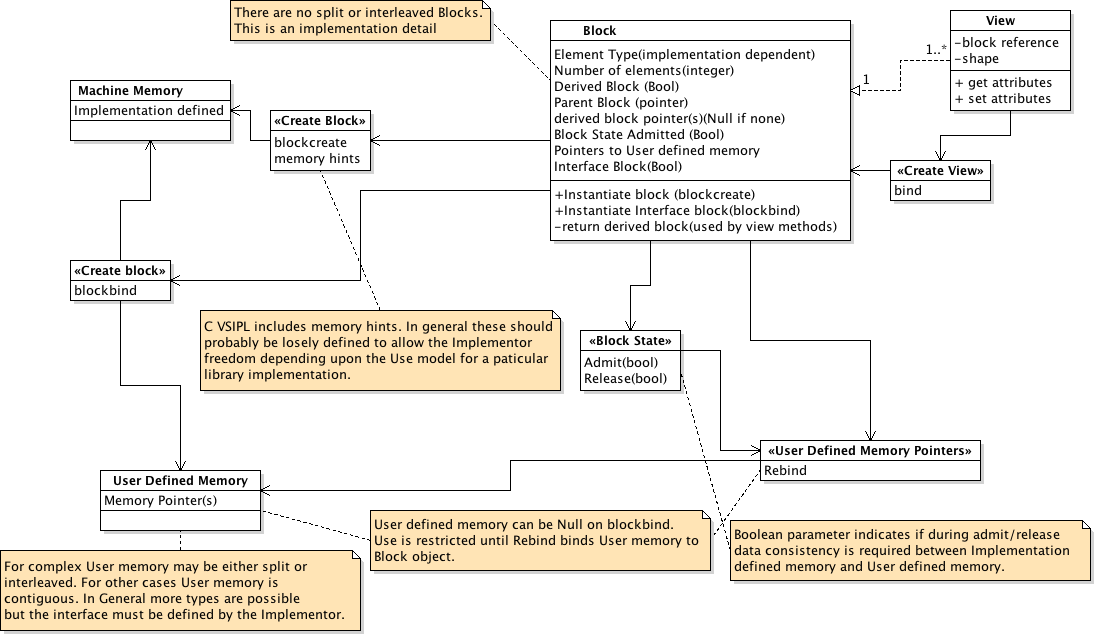
\includegraphics[width=.7\textwidth]{./InterfaceBlockMemoryRelationship}
\captionof{figure}{Memory, Block and View Relation}
\label{fig:MemoryBlockView}
\end{minipage}
\begin{minipage}[c]{1.1\textwidth}
\centering
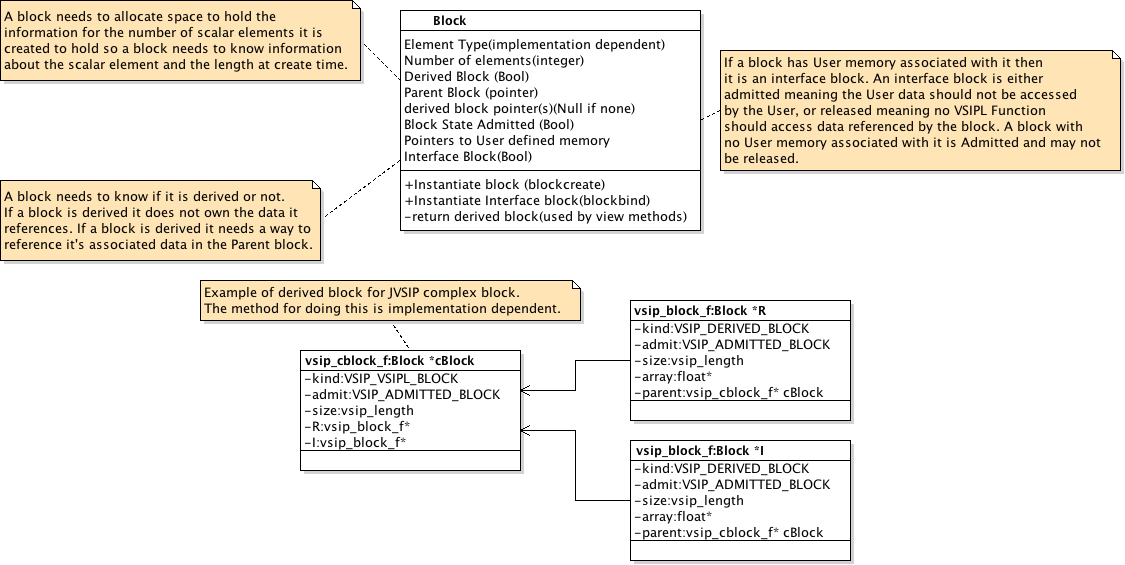
\includegraphics[width=1.05\textwidth]{./BlockBasicsOne}
\captionof{figure}{Basic Block Class for \cvl{} and Example Showing Complex and Derived Block for \jv{} \cvl{} \\[12pt]}
\label{fig:BasicBlockOne}
\end{minipage}
\begin{minipage}[c]{1\textwidth}
\centering
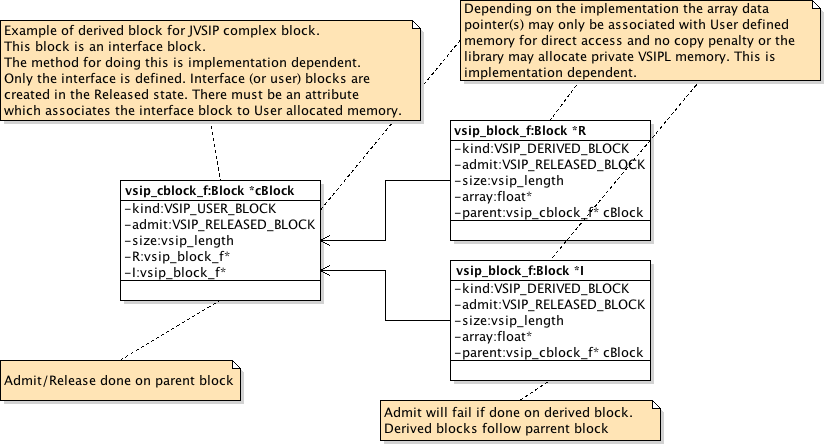
\includegraphics[width=.7\textwidth]{./BlockBasicsTwo}
\captionof{figure}{Basic Block Showing Complex and Derived \jv{} \blk{} for \cvl{} Interface \blk{}}
\label{fig:BasicBlockTwo}
\end{minipage}
\begin{minipage}[c]{1\textwidth}
\centering
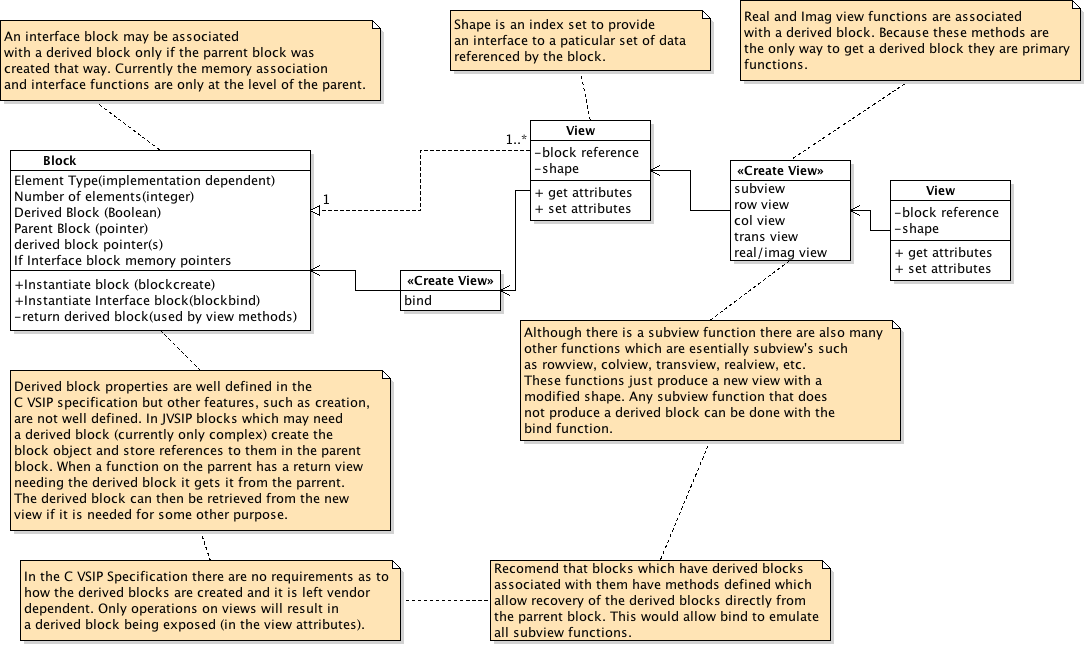
\includegraphics[width=.7\textwidth]{./BlockViewRelationshipDerived}
\captionof{figure}{Block and View and Subview Relation}
\label{fig:BlockViewSubview}
\end{minipage}
\end{document}


